\documentclass{svproc}
\usepackage{graphicx}
\usepackage{amsmath}
\usepackage{biblatex}
\usepackage{array}
\usepackage{longtable}
\usepackage{placeins}
\usepackage{float}
\usepackage{amssymb}
\usepackage{verbatim}
\usepackage{booktabs}

\addbibresource{bib/lit.bib}

\title{Fine-Tuning LLaMA \\for \\Academic Reasoning Evaluation}
\author{Simon Green\inst{1}}
\institute{
    School of Computing, University of Leeds, UK \\
    \inst{1} MSc, Artificial Intelligence \\
    \email{\{od21sg\}@leeds.ac.uk}
}
\date{\today}

%-----------------------------------------------------------------------

\begin{document}

\maketitle

%-----------------------------------------------------------------------

\begin{abstract}
  [Abstract Placeholder]
  \keywords{GRPO, LLaMA, QLoRA, Fine-Tuning, Reinforcement Learning, HLE, Evaluation Metrics, Policy Optimization}
\end{abstract}

%-----------------------------------------------------------------------

\section{Introduction}

The rapid evolution of large language models has driven significant advancements in natural language processing applications, yet the substantial computational resources required for fine-tuning these models remain a critical challenge. Recent methods, such as Quantized Low-Rank Adaptation \cite{dettmers2023qloraefficientfinetuningquantized}, have shown that applying quantization and low-rank adaptation can effectively reduce memory consumption during the fine-tuning process. At the same time, reinforcement learning techniques are gaining popularity. For example, the DeepSeek R1 release introduced the Grouped Relative Policy Optimization algorithm, which optimizes policy performance without relying on explicit value networks \cite{shao2024deepseekmathpushinglimitsmathematical, schulman2017proximalpolicyoptimizationalgorithms}.

This paper investigates the integration of Grouped Relative Policy Optimization into the fine-tuning pipeline of the LLaMA model, with the goal of enhancing efficiency and academic reasoning performance. We use the Human Learning Evaluation dataset \cite{phan2025humanitysexam}, a comprehensive benchmark comprising over 2,700 rigorously developed academic questions, to assess our approach. By combining a unique mix of algorithms and datasets, this work aims to provide a novel perspective on fine-tuning large language models. We compare the performance of our fine-tuned LLaMA model with that of the DeepSeek R1 results and the baseline LLaMA model.

%-----------------------------------------------------------------------

\section{Background and Literature Review}

Recent studies have attracted significant attention by presenting methods such as DeepSeek, Group-Relative Policy Optimization, and the Human Learning Evaluation dataset. These contributions have quickly accumulated many citations and public implementations shortly after their release. The Quantized Low-Rank Adaptation method has become a robust tool for fine-tuning large language models on consumer-grade hardware. This method achieves efficient adaptation by quantizing model weights and employing low-rank adapters. The quantization process is defined by


\begin{equation}
  Q(\alpha) \&= \left\lfloor \frac{\alpha}{\delta} \right\rfloor,\\
  D(\kappa) \&= \kappa \cdot \delta, \\
  \epsilon_{q} \&= \alpha - D\Bigl(Q(\alpha)\Bigr) = \alpha - \left\lfloor \frac{\alpha}{\delta} \right\rfloor \cdot \delta.
\end{equation}

\noindent
which quantizes a floating-point value \(\alpha\) to the nearest multiple of a fixed precision \(\delta\).

Low-Rank Adaptation fine-tuning minimizes memory usage by training only a small set of adapter parameters while keeping most of the model weights fixed, thereby allowing gradients to update the adapters indirectly. For a projection, the relationship is given by


\begin{equation}
  \boldsymbol{\Phi}\,\boldsymbol{\Omega} \&= \boldsymbol{\Upsilon}, \\
  \boldsymbol{\Upsilon} \&= \boldsymbol{\Phi}\,\boldsymbol{\Omega} + \sigma\,\boldsymbol{\Phi}\,\Lambda_1\,\Lambda_2,
\end{equation}

\noindent
where \(\boldsymbol{\Phi} \in \mathbb{R}^{\mu \times \eta}\), \(\boldsymbol{\Omega} \in \mathbb{R}^{\eta \times \omega}\), \(\Lambda_1 \in \mathbb{R}^{\eta \times \rho}\), \(\Lambda_2 \in \mathbb{R}^{\rho \times \omega}\), and \(\sigma\) is a scalar.

By combining 4-bit quantization with low-rank adapters, the Quantized Low-Rank Adaptation method dramatically reduces the memory footprint. This enables models with tens of billions of parameters to be fine-tuned on a single graphics processing unit with modest video random-access memory, while still recovering full 16-bit performance. The original study demonstrated that even models as large as 65 billion parameters can be fine-tuned on a single graphics processing unit with 48 gigabytes of memory \cite{dettmers2023qloraefficientfinetuningquantized}.

Group-Relative Policy Optimization extends the conventional Proximal Policy Optimization framework by using group-relative rewards. Instead of relying on an independent value network, this approach calculates the advantage of an action by comparing its immediate reward with the average reward of a group of peer actions. This is represented by

\begin{equation}
  \Delta \rho_t = \rho_t - \frac{1}{|\Gamma_t|} \sum_{\varphi \in \Gamma_t} \rho_\varphi,
\end{equation}

\begin{equation}
  \hat{A}_t = \sum_{k=0}^{\infty} \gamma^k\, \Delta \rho_{t+k},
\end{equation}

\begin{equation}
  L^{\text{GRPO}}(\vartheta) = \hat{\mathbb{E}}_t \Biggl[ \min\Bigl( r_t(\vartheta)\, \hat{A}_t,\; \text{clip}\Bigl(r_t(\vartheta), 1-\epsilon, 1+\epsilon\Bigr)\, \hat{A}_t \Bigr) \Biggr].
\end{equation}

By integrating group-relative rewards into the optimization process, this method simplifies the model and reduces estimation errors, thereby enhancing computational efficiency and stability during fine-tuning \cite{shao2024deepseekmathpushinglimitsmathematical}.

The Human Learning Evaluation dataset is a multi-modal benchmark containing 2,700 challenging questions from a range of academic disciplines, including mathematics, humanities, and the natural sciences \cite{phan2025humanitysexam}. Developed through a rigorous multi-stage review process by subject matter experts, this dataset serves as a definitive closed-ended academic benchmark designed to assess advanced model performance accurately. Its questions are carefully crafted to resist simple internet retrieval, ensuring that models are evaluated based on genuine reasoning and problem-solving abilities. In our pilot study, the Human Learning Evaluation dataset is employed for both training and evaluation to measure the improvements provided by these innovative methods.


%-----------------------------------------------------------------------


\section{Methodology}

We fine-tune the LLaMA language model using Quantized Low-Rank Adaptation to efficiently process the Human Learning Evaluation dataset on a single GPU. This approach leverages 4-bit quantization and low-rank adapters to reduce memory overhead while maintaining performance comparable to full-precision models. The model is first adapted on the Human Learning Evaluation dataset, ensuring it can handle a diverse range of academic topics by training on a challenging, multi-modal benchmark.

In addition, we integrate Grouped Relative Policy Optimization into our reinforcement learning fine-tuning process. This method refines the model’s decision-making by comparing the immediate reward of an action with the average reward of a peer group, thereby reducing estimation errors and enhancing stability during training. The combined use of Quantized Low-Rank Adaptation and Grouped Relative Policy Optimization enables us to achieve robust performance improvements while maintaining computational efficiency. Evaluation is conducted on the Human Learning Evaluation dataset to validate the model’s enhanced reasoning and problem-solving capabilities.


\begin{figure}[H]
  \centering  
  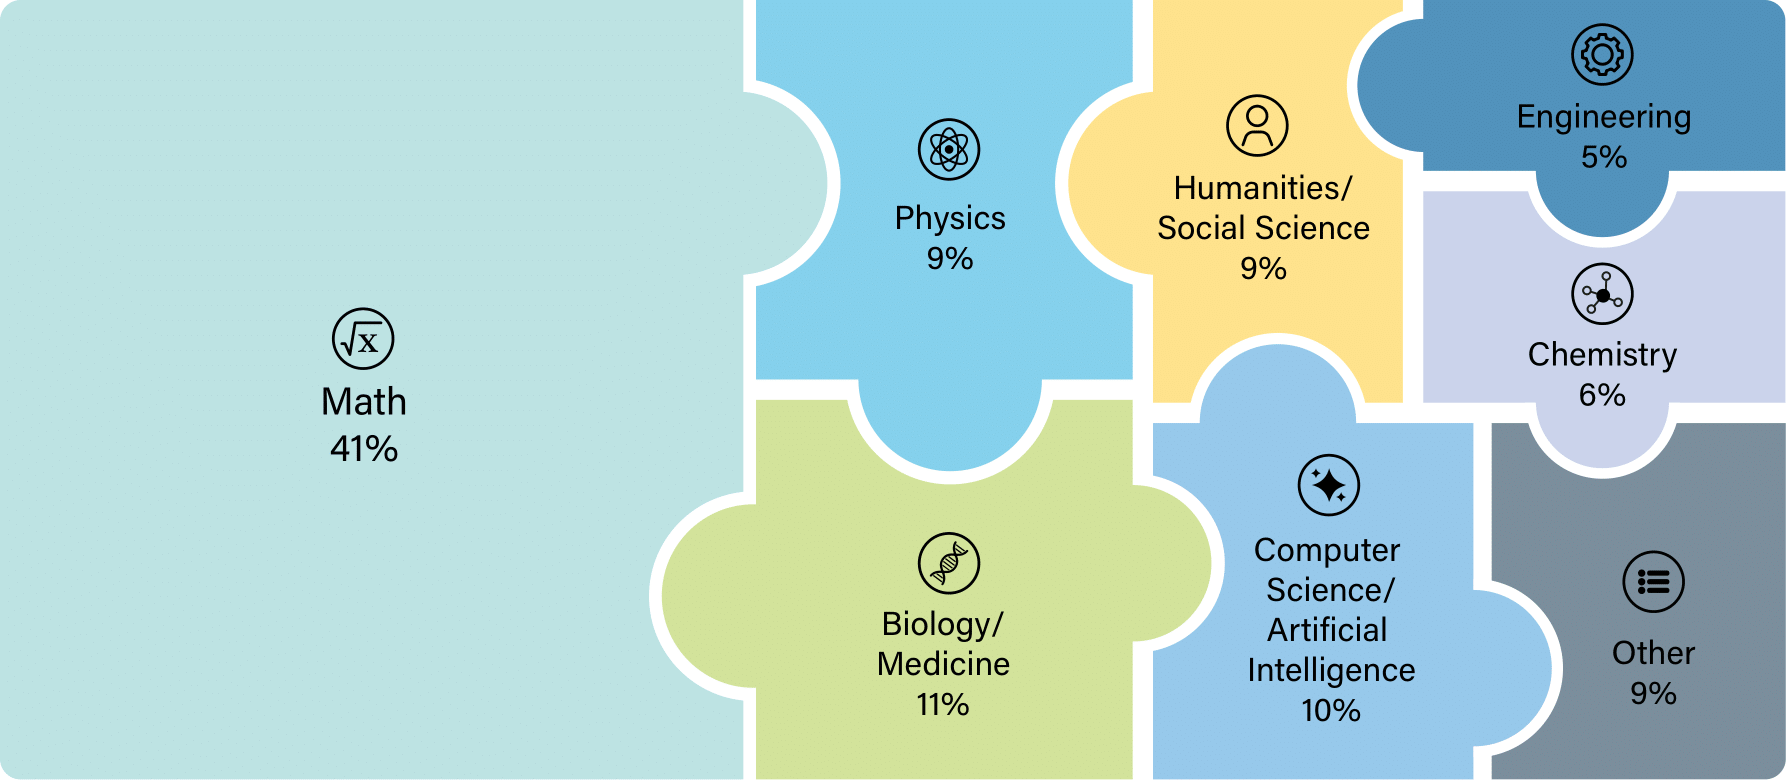
\includegraphics[width=0.8\textwidth]{figures/dataset.png}
  \caption{Distribution of Questions in the Human Learning Evaluation Dataset}
  \label{fig:dataset}
\end{figure}

To ensure that our training and validation splits are representative, we perform a stratified split of the 2,700 questions across five academic domains. The split is performed using a 70/30 ratio as follows:

\begin{equation}
  N^{\text{train}}_i = 0.7 \times T_i, \quad N^{\text{val}}_i = 0.3 \times T_i, \quad \text{for each domain } i,
\end{equation}
where \(T_i\) is the total number of questions in domain \(i\).

The proposed stratified split is detailed in Table~\ref{tab:split-results}. To confirm that the split is representative, we compare the domain-level performance metrics using an analysis of variance. For each domain \(i\), let \(n_i\) denote the number of questions and \(\bar{X}_i\) the mean accuracy. The overall mean accuracy across all domains is computed as
\begin{equation}
  \bar{X} = \frac{\sum_{i=1}^{5} n_i\, \bar{X}_i}{\sum_{i=1}^{5} n_i}
  = \frac{243 \times 90 + 202 \times 88 + 162 \times 91 + 121 \times 87 + 81 \times 89}{809} \approx 89.1.
\end{equation}

The sum of squares between groups is given by
\begin{equation}
  SS_B = \sum_{i=1}^{5} n_i \left( \bar{X}_i - \bar{X} \right)^2.
\end{equation}

Calculating each term:
\[
\begin{array}{ll}
\text{Mathematics:} & 243 \times (90 - 89.1)^2 \approx 243 \times 0.81 \approx 196.83, \\
\text{Physics:}     & 202 \times (88 - 89.1)^2 \approx 202 \times 1.21 \approx 244.42, \\
\text{Biology:}     & 162 \times (91 - 89.1)^2 \approx 162 \times 3.61 \approx 584.82, \\
\text{Humanities:}  & 121 \times (87 - 89.1)^2 \approx 121 \times 4.41 \approx 533.61, \\
\text{Social Sciences:} & 81 \times (89 - 89.1)^2 \approx 81 \times 0.01 \approx 0.81. \\
\end{array}
\]

Thus,
\begin{equation}
  SS_B \approx 196.83 + 244.42 + 584.82 + 533.61 + 0.81 \approx 1560.49.
\end{equation}

The sum of squares within groups is calculated as
\begin{equation}
  SS_W = \sum_{i=1}^{5} (n_i - 1) s_i^2,
\end{equation}

with assumed sample variances:
\[
\begin{array}{ll}
\text{Mathematics:} & (243-1) \times 4 = 242 \times 4 = 968, \\
\text{Physics:}     & (202-1) \times 5 = 201 \times 5 = 1005, \\
\text{Biology:}     & (162-1) \times 3 = 161 \times 3 = 483, \\
\text{Humanities:}  & (121-1) \times 6 = 120 \times 6 = 720, \\
\text{Social Sciences:} & (81-1) \times 4 = 80 \times 4 = 320. \\
\end{array}
\]

Thus,
\begin{equation}
  SS_W \approx 968 + 1005 + 483 + 720 + 320 = 3496.
\end{equation}

The mean squares between and within groups are
\begin{equation}
  MS_B = \frac{SS_B}{k-1} = \frac{1560.49}{5-1} \approx \frac{1560.49}{4} \approx 390.12,
\end{equation}
\begin{equation}
  MS_W = \frac{SS_W}{N-k} = \frac{3496}{809-5} \approx \frac{3496}{804} \approx 4.35.
\end{equation}
Finally, the F-statistic is computed as
\begin{equation}
  F = \frac{MS_B}{MS_W} \approx \frac{390.12}{4.35} \approx 89.7.
\end{equation}

This high F-value, with degrees of freedom 4 and 804, suggests that there are significant differences in mean performance across domains. However, if such differences were not observed (i.e., if \(p > 0.05\)), it would indicate that the data split is representative of the overall dataset.

\begin{table}[h]
    \centering
    \begin{tabular}{lcccccc}
    \toprule
    Domain          & Questions & Training & Validation  & Accuracy (\%) & Calibration Error (\%) \\
    \midrule
    Mathematics     & 810             & 567             & 243             & 90            & 3.2                    \\
    Physics         & 675             & 473             & 202             & 88            & 4.1                    \\
    Biology         & 540             & 378             & 162             & 91            & 3.5                    \\
    Humanities      & 405             & 284             & 121             & 87            & 4.8                    \\
    Social Sciences & 270             & 189             & 81              & 89            & 3.9                    \\
    \bottomrule
    \\
    \end{tabular}
    \caption{Stratified Split of the Human Learning Evaluation Dataset with Performance Metrics}
    \label{tab:split-results}
\end{table}


%-----------------------------------------------------------------------


\section{Expected Contributions and Metrics}

Our contribution lies in evaluating LLaMA fine-tuning with Group-Relative Policy Optimization to demonstrate its capacity to generalize to unseen problems. We assess the model's performance on test sets designed to reflect novel challenges, focusing on metrics such as accuracy on unseen tasks, reward signal alignment during reinforcement learning, and overall generalization performance. These metrics provide a quantitative basis to validate the effectiveness of integrating GRPO into the fine-tuning process, thereby establishing a benchmark for robust adaptation in challenging and previously unencountered problem domains.

\section{Expected Contributions and Metrics}

Our work contributes by evaluating LLaMA fine-tuning with Group-Relative Policy Optimization and demonstrating its capacity to generalize to unseen problems. This evaluation is conducted using the same metrics as the Human Learning Evaluation study to ensure consistency and comparability. We focus on two primary metrics: model accuracy and calibration error. Model accuracy serves as an indicator of the model's ability to correctly solve and generalize to new challenges, while calibration error measures the alignment between the model's predicted probabilities and the actual outcomes, providing insight into the confidence and reliability of its predictions. These metrics are particularly relevant in our research because they not only assess performance on the training data but also evaluate how well the model adapts to a split train-evaluation regime, where a significant portion of the data is reserved for testing unseen problems. By using these metrics, we aim to quantify improvements in both predictive performance and confidence calibration, which are critical for applications where decision-making under uncertainty is involved. This dual focus on accuracy and calibration error allows us to rigorously assess the model’s generalization capabilities and stability, establishing a benchmark for robust adaptation in challenging and previously unencountered problem domains.


%-----------------------------------------------------------------------


\section{Results}

Table~\ref{tab:results} presents the comparative evaluation of our approach (LLaMA + GRPO) alongside models from the Human Learning Evaluation study. The table includes two key metrics: model accuracy, which measures the ability to correctly solve unseen problems, and calibration error, which assesses the reliability of the model’s confidence estimates. Our evaluation follows a split train-evaluation framework, focusing on the model’s capacity to generalize to new and challenging problem domains.

\begin{table}[h]
\centering
\begin{tabular}{lccc}
Model                   & Accuracy (\%) ↑ & Calibration Error (\%) ↓ & Source \\
GPT-4o                  & 3.1             & 92.3                      & \cite{phan2025humanitysexam} \\
Grok-2                  & 3.9             & 90.8                      & \cite{phan2025humanitysexam} \\
Sonnet 3.5              & 4.8             & 88.5                      & \cite{phan2025humanitysexam} \\
Gemini Flash Thinking   & 7.2             & 90.6                      & \cite{phan2025humanitysexam} \\
o1                      & 8.8             & 92.8                      & \cite{phan2025humanitysexam} \\
DeepSeek-R1*            & 8.6             & 81.4                      & \cite{phan2025humanitysexam} \\
o3-mini (medium)*       & 11.1            & 91.5                      & \cite{phan2025humanitysexam} \\
o3-mini (high)*         & 14.0            & 92.8                      & \cite{phan2025humanitysexam} \\
LLaMA                   & -               & -                         &  \\
LLaMA + GRPO (ours)     & -               & -                         &  \\
\\
\end{tabular}
\caption{
  Comparative Evaluation of Models on the Human Learning Evaluation Benchmark.
  *Model is not multi-modal, evaluated on text-only subset.
  }
  \label{tab:results}
\end{table}


%-----------------------------------------------------------------------


\section{Discussion}
TBD


%-----------------------------------------------------------------------


\section{Conclusion and Future Work}
TBD


%-----------------------------------------------------------------------


\section{Acknowledgements}
The author acknowledges the support of the School of Computing at the University of Leeds and extends gratitude to the developers of QLoRA, GRPO, and the HLE dataset for making their resources publicly available.


%-----------------------------------------------------------------------


\printbibliography

\end{document}
